% ==============================================================================
%  Análise Bibliométrica da Produção Acadêmica do C4AI (USP)
%  Documento gerado a partir das figuras em figuras/
%  Compilar com: pdflatex documento_analise.tex
% ==============================================================================
\documentclass[12pt,a4paper]{article}

% ── Codificação e idioma ──────────────────────────────────────────────────────
\usepackage[utf8]{inputenc}
\usepackage[T1]{fontenc}
\usepackage[brazil]{babel}

% ── Layout ────────────────────────────────────────────────────────────────────
\usepackage[margin=2.5cm]{geometry}
\usepackage{graphicx}
\usepackage{float}
\usepackage{booktabs}
\usepackage{caption}
\usepackage{subcaption}
\usepackage{xcolor}
\usepackage{microtype}
\usepackage{siunitx}
\usepackage{hyperref}

\hypersetup{
    colorlinks=true,
    linkcolor=blue!50!black,
    citecolor=blue!50!black,
    urlcolor=blue!50!black,
}

% Diretório das figuras
\graphicspath{{figuras/}}

% Estilo das legendas
\captionsetup{
    font=small,
    labelfont=bf,
    textfont=it,
    justification=justified,
    width=0.95\textwidth,
}

% ── Metadados ─────────────────────────────────────────────────────────────────
\title{\textbf{Análise Bibliométrica da Produção Acadêmica do C4AI}\\[0.3em]
       \large Centro de Inteligência Artificial da Universidade de São Paulo\\
       \normalsize (USP \textbullet{} FAPESP \textbullet{} IBM)}
\author{Pesquisa etnográfica do C4AI --- Doutorado em Ciências Sociais (IFCH/Unicamp)}
\date{Período analisado: 2020--2024}

% ==============================================================================
\begin{document}

\maketitle

\begin{abstract}
\noindent
Este documento apresenta uma análise bibliométrica exploratória da produção
acadêmica dos oito grupos de pesquisa que compõem o \textbf{Centro de
Inteligência Artificial da Universidade de São Paulo (C4AI)}: Agribio, AI
HEALTH, KEML, MClimate, NLP2, OceanML, PROINDL e HUMANITIES. Foram contabilizadas
\textbf{569 publicações} no período de \textbf{2020 a 2024}. As análises abrangem
o \emph{ranking} e a distribuição proporcional por grupo, a evolução temporal
agregada e por grupo, a taxa de produtividade (publicações por ano) e indicadores
de concentração da produção (índice Herfindahl--Hirschman, HHI). Os resultados
indicam uma produção fortemente concentrada --- os três maiores grupos respondem
por \textbf{68{,}4\%} de todas as publicações --- com pico de produção em
\textbf{2023} (313 publicações) e liderança consolidada do grupo AI HEALTH.
\end{abstract}

\tableofcontents
\bigskip

% ==============================================================================
\section{Introdução e metodologia}
% ==============================================================================

A análise consolida as planilhas de publicações dos grupos de pesquisa do C4AI
em um único conjunto de dados limpo. Após a normalização das colunas
(\texttt{Grupo}, \texttt{Ano}, \texttt{Título}) e a remoção de registros
inválidos, restaram \num{569} publicações distribuídas entre \num{8} grupos no
intervalo de \num{2020} a \num{2024}. As métricas e visualizações foram geradas
com as bibliotecas \texttt{pandas}, \texttt{matplotlib} e \texttt{seaborn}.

\begin{table}[H]
\centering
\caption{Indicadores gerais da produção acadêmica do C4AI no período analisado.}
\label{tab:indicadores}
\begin{tabular}{lr}
\toprule
\textbf{Indicador} & \textbf{Valor} \\
\midrule
Total de publicações                     & \num{569} \\
Período analisado                        & 2020--2024 \\
Número de grupos de pesquisa             & \num{8} \\
Média geral de publicações por ano       & \num{113.8} \\
Ano mais produtivo                       & 2023 (\num{313} pubs) \\
Grupo mais produtivo (total)             & AI HEALTH (\num{200} pubs) \\
Grupo mais eficiente (pubs/ano)          & AI HEALTH (\num{50.00}) \\
Concentração nos 3 maiores grupos        & \SI{68.4}{\percent} \\
Índice de concentração HHI               & \num{2104} (moderado) \\
\bottomrule
\end{tabular}
\end{table}

% ==============================================================================
\section{Distribuição da produção por grupo}
% ==============================================================================

% ── Figura 1: Ranking ─────────────────────────────────────────────────────────
\begin{figure}[H]
\centering
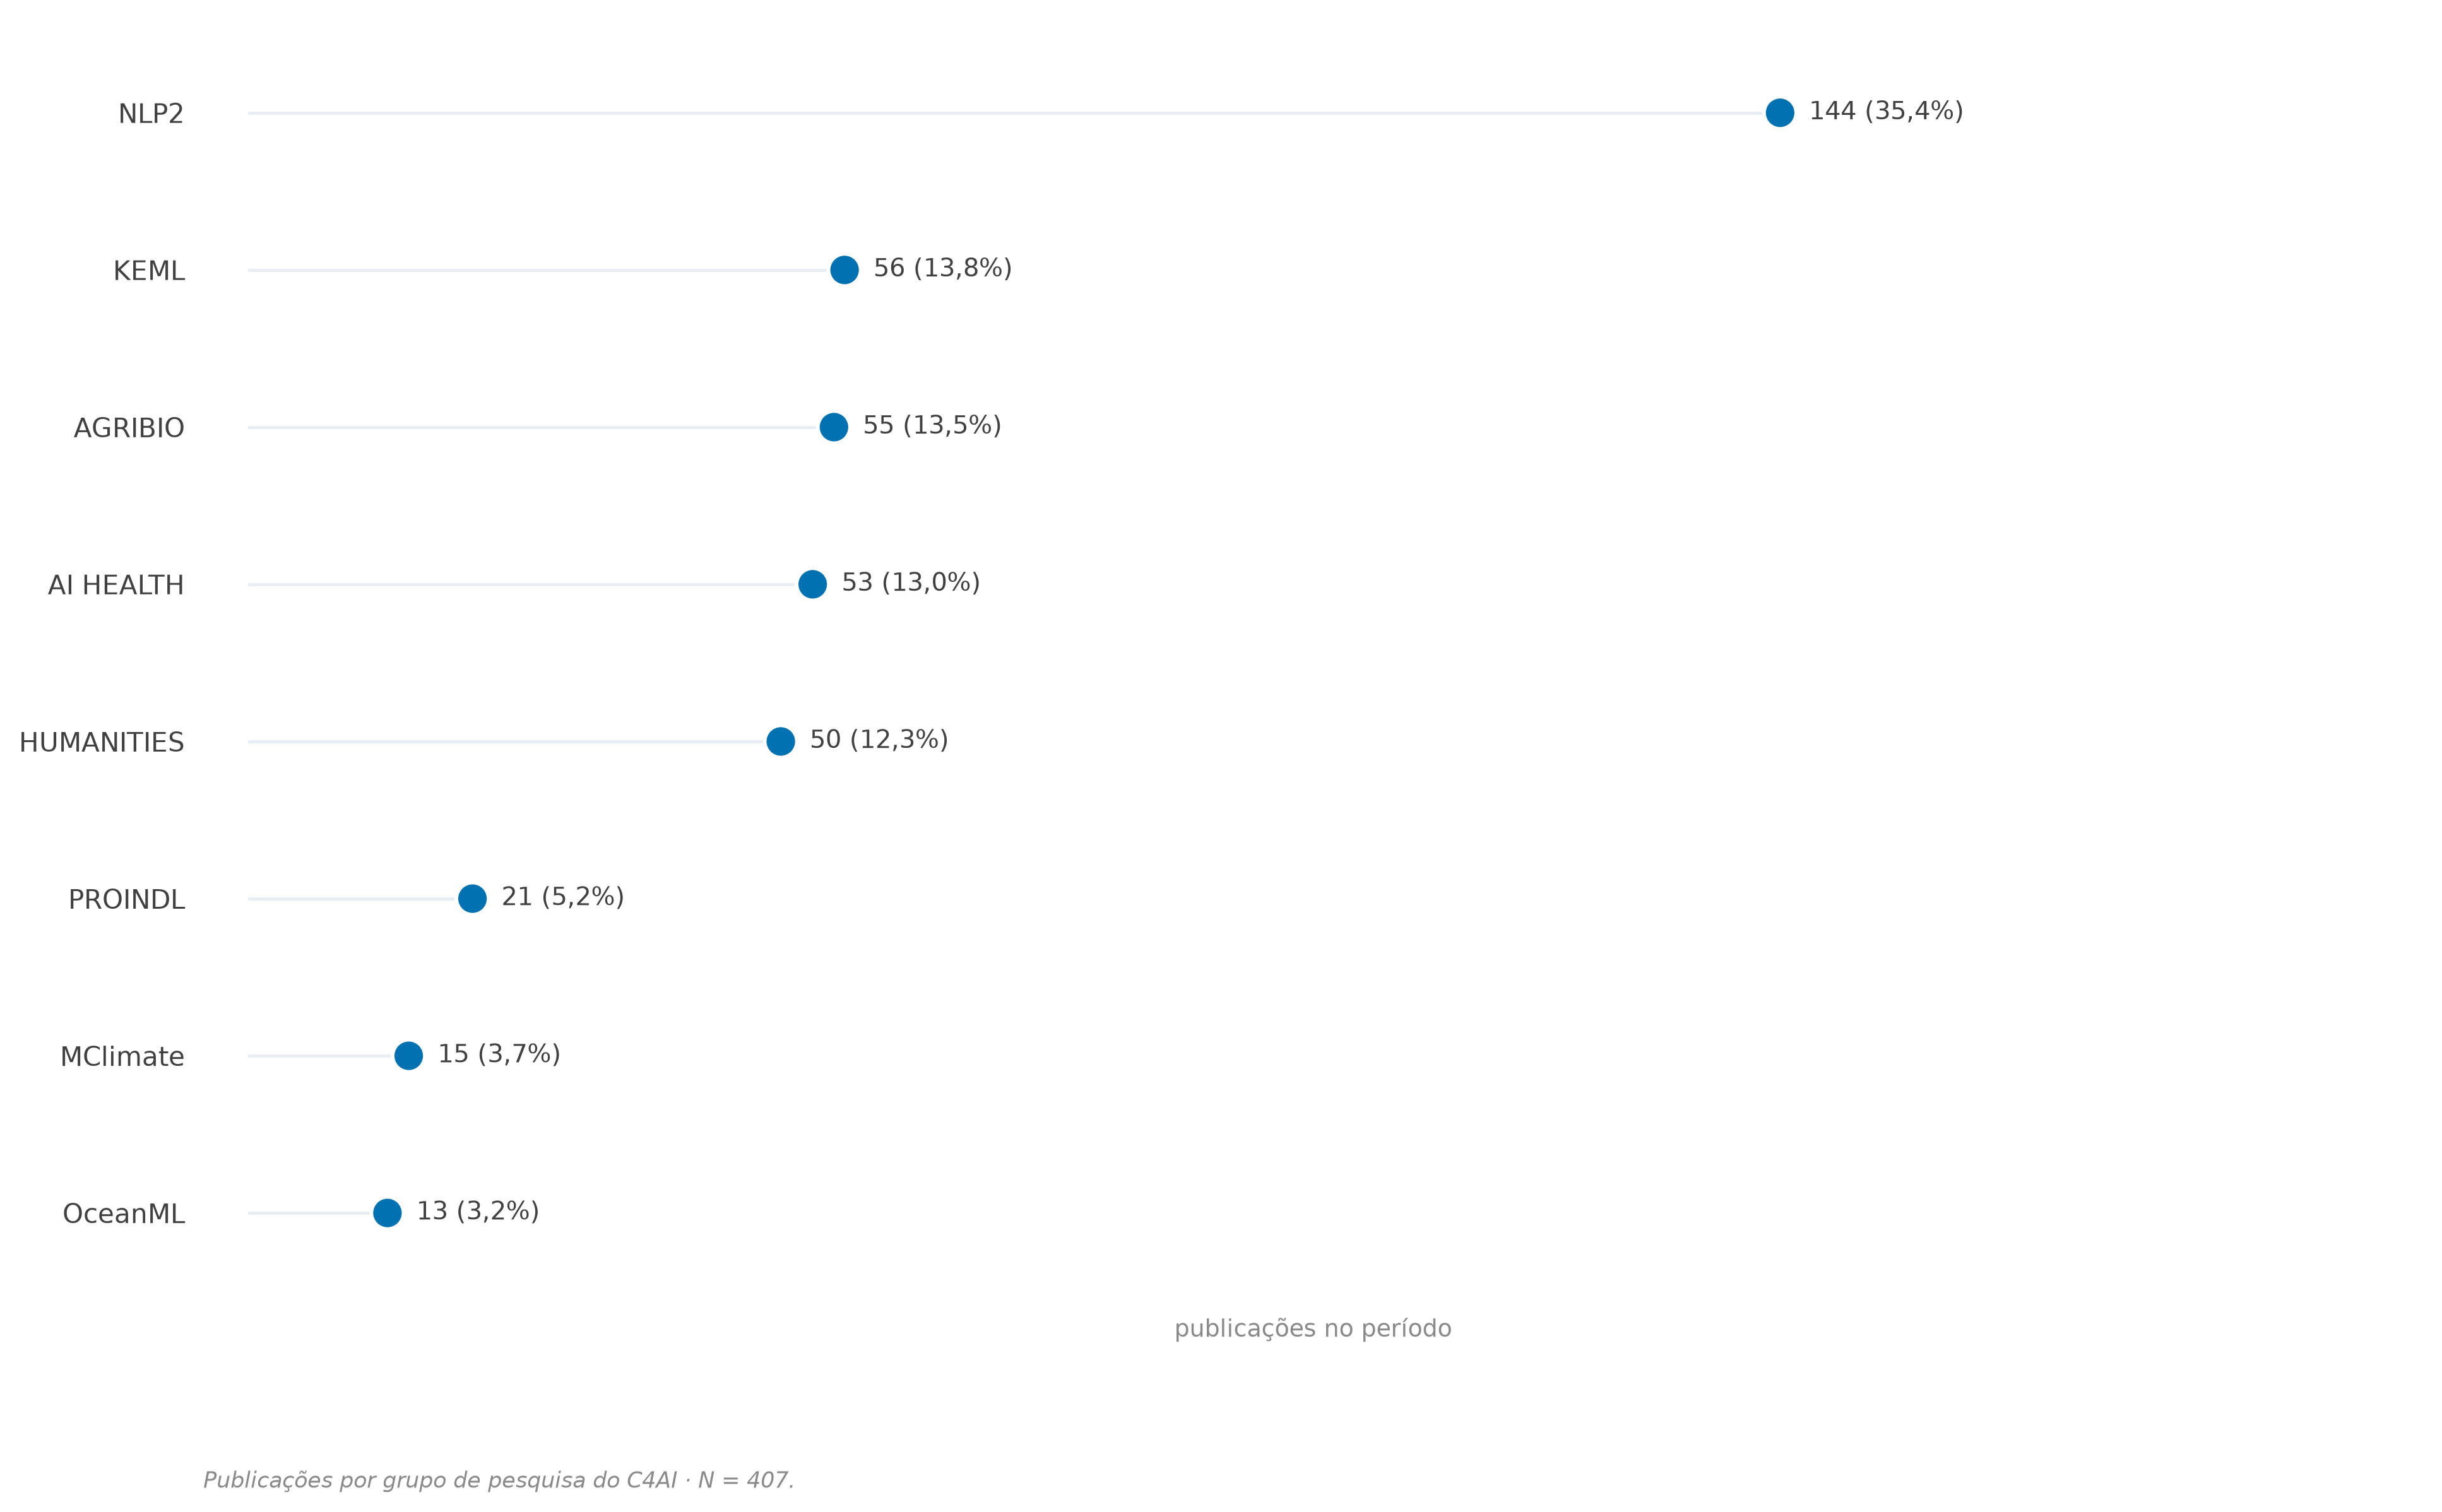
\includegraphics[width=0.92\textwidth]{1_ranking_grupos.png}
\caption[Ranking de publicações por grupo]{%
\textbf{Ranking de publicações por grupo de pesquisa do C4AI.}
Gráfico de barras horizontais ordenado de forma decrescente pelo número absoluto
de publicações. O grupo \textbf{AI HEALTH} lidera com \num{200} publicações
(\SI{35.1}{\percent} do total), seguido por \textbf{NLP2} com \num{131}
(\SI{23.0}{\percent}). Os demais grupos --- Agribio (\num{58}; \SI{10.2}{\percent}),
KEML (\num{55}; \SI{9.7}{\percent}), HUMANITIES (\num{47}; \SI{8.3}{\percent}),
PROINDL (\num{40}; \SI{7.0}{\percent}), OceanML (\num{23}; \SI{4.0}{\percent}) e
MClimate (\num{15}; \SI{2.6}{\percent}) --- apresentam volumes substancialmente
menores, evidenciando a assimetria da produção entre os grupos.}
\label{fig:ranking}
\end{figure}

% ── Figura 2: Pizza ───────────────────────────────────────────────────────────
\begin{figure}[H]
\centering
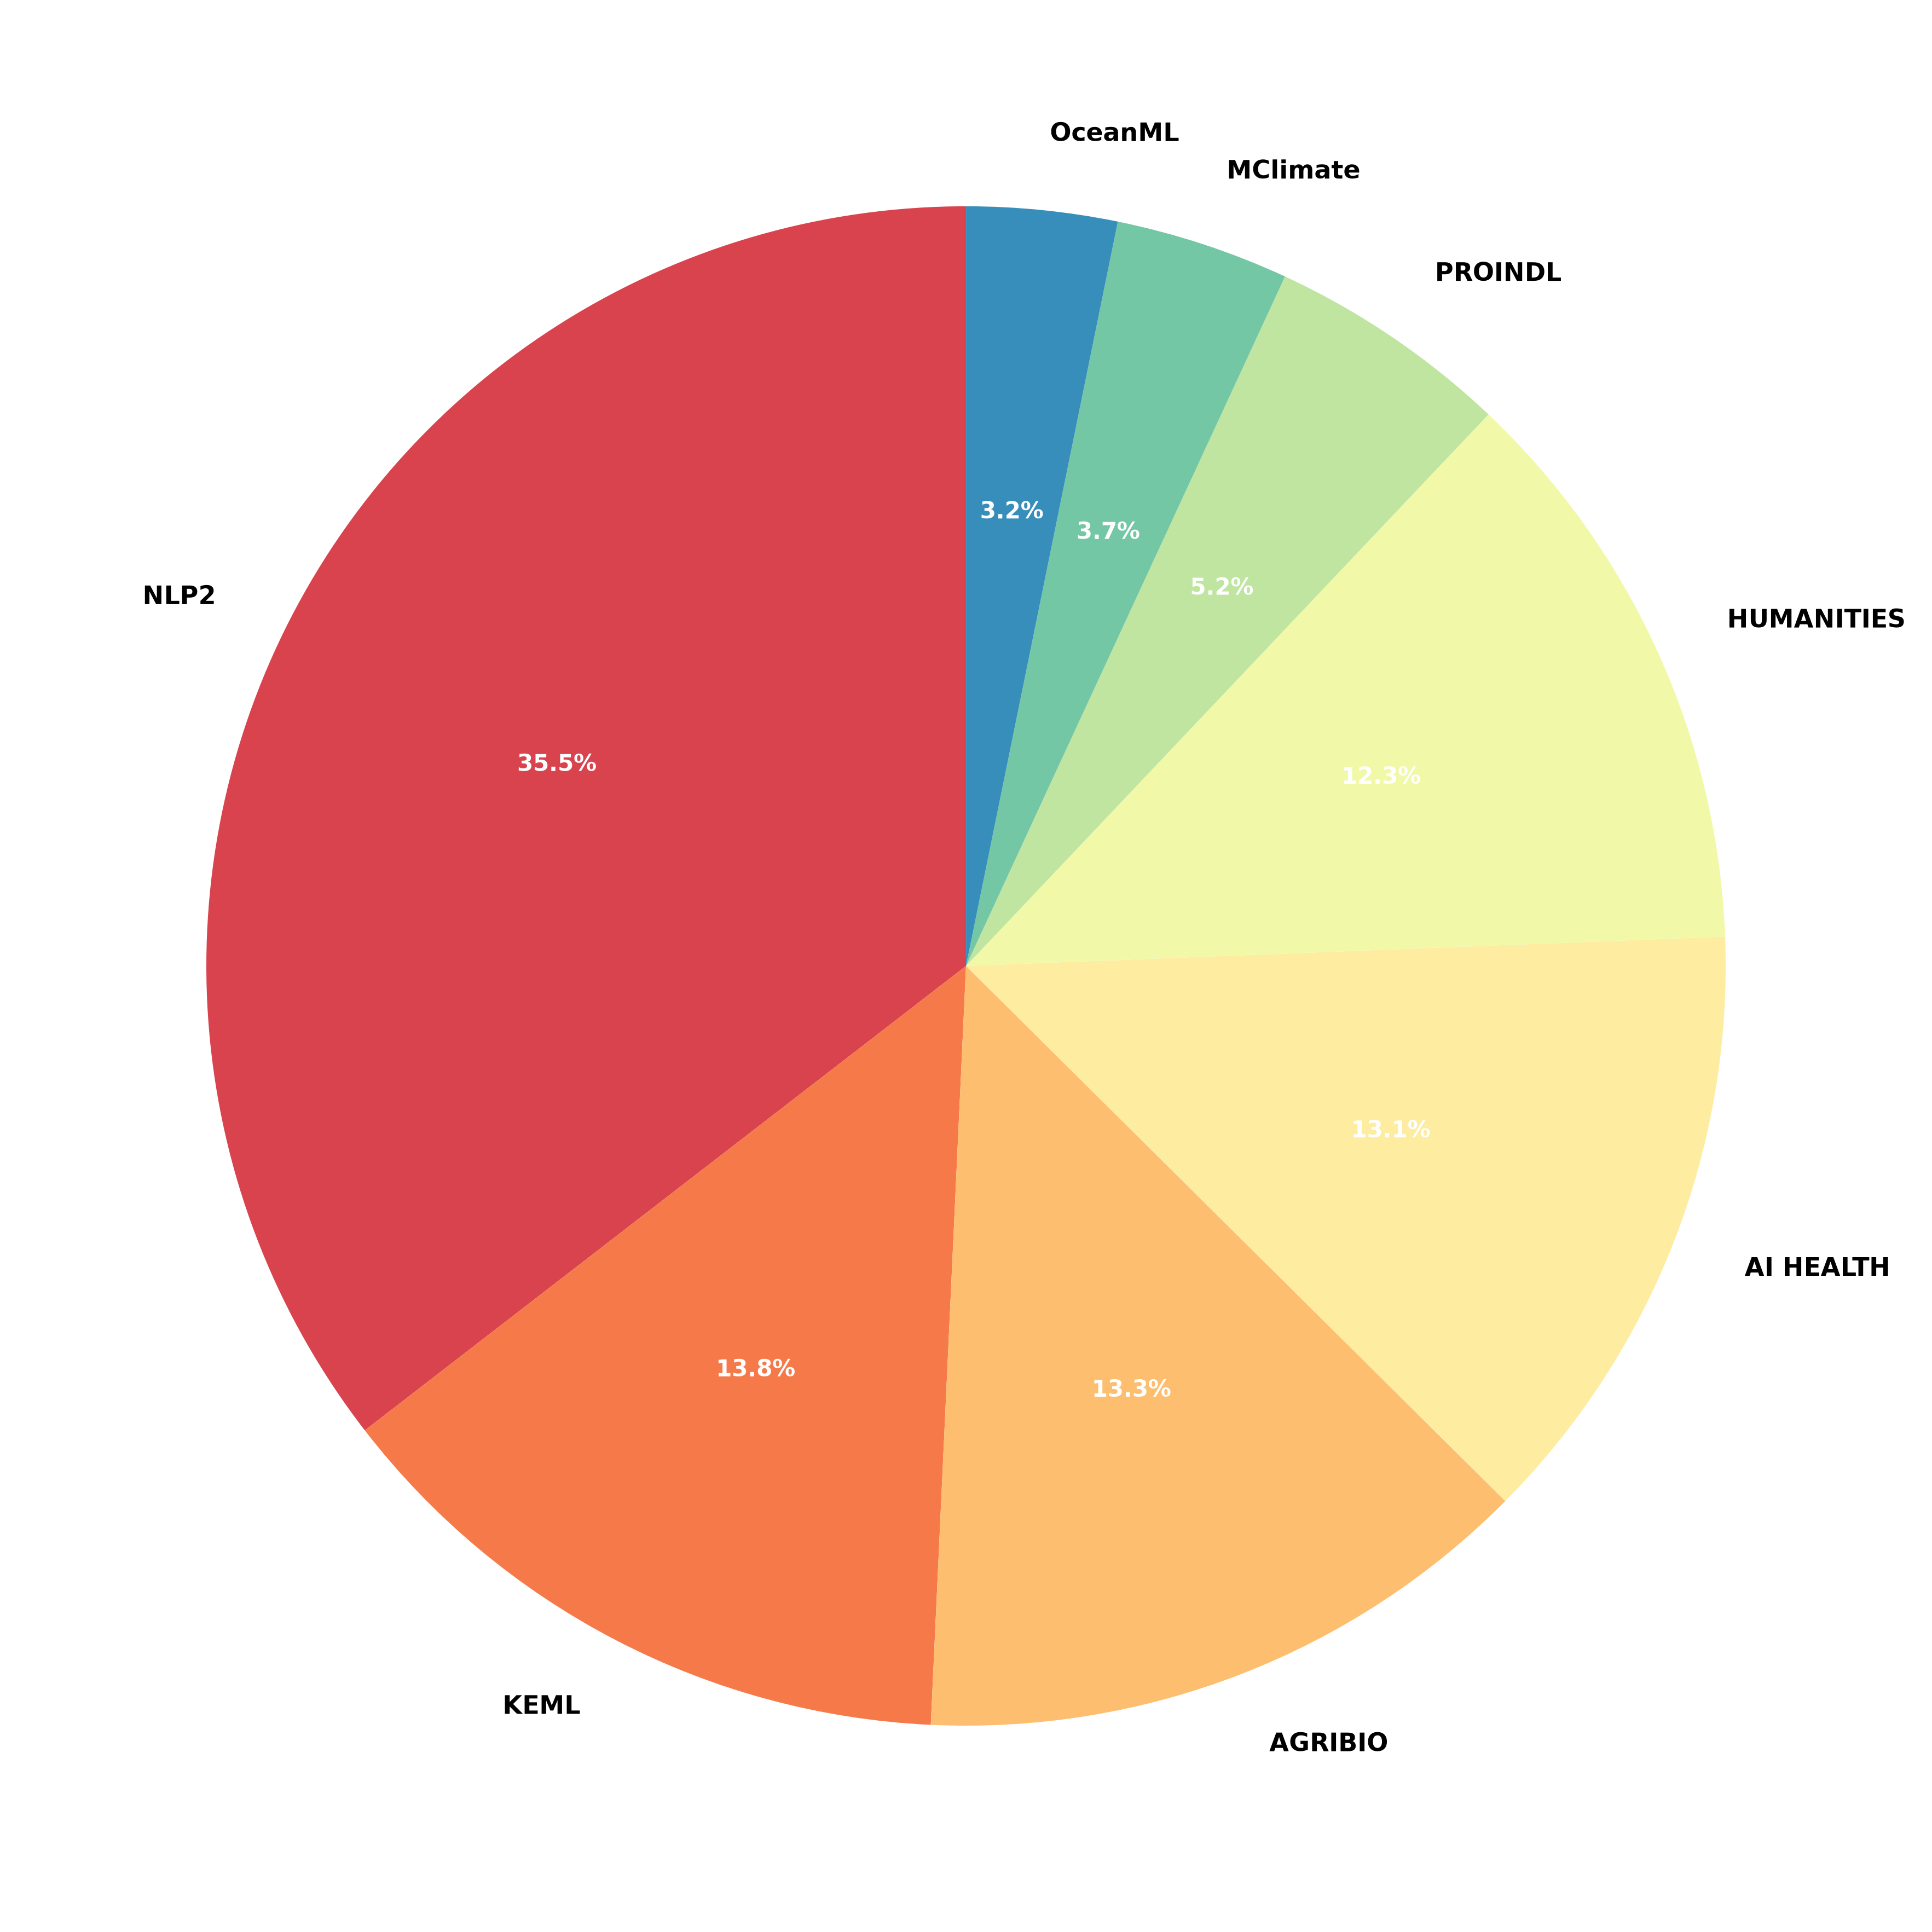
\includegraphics[width=0.75\textwidth]{2_pizza_grupos.png}
\caption[Distribuição proporcional por grupo]{%
\textbf{Distribuição proporcional de publicações por grupo.}
O gráfico de setores reforça a leitura do ranking (Figura~\ref{fig:ranking}),
destacando que AI HEALTH e NLP2 somam, juntos, mais da metade da produção
(\SI{58.1}{\percent}). A fatia dos cinco grupos menores --- de Agribio a
MClimate --- corresponde a menos de um terço do total, ilustrando a
concentração da produção em poucos grupos.}
\label{fig:pizza}
\end{figure}

% ==============================================================================
\section{Evolução temporal da produção}
% ==============================================================================

% ── Figura 3: Evolução temporal geral ─────────────────────────────────────────
\begin{figure}[H]
\centering
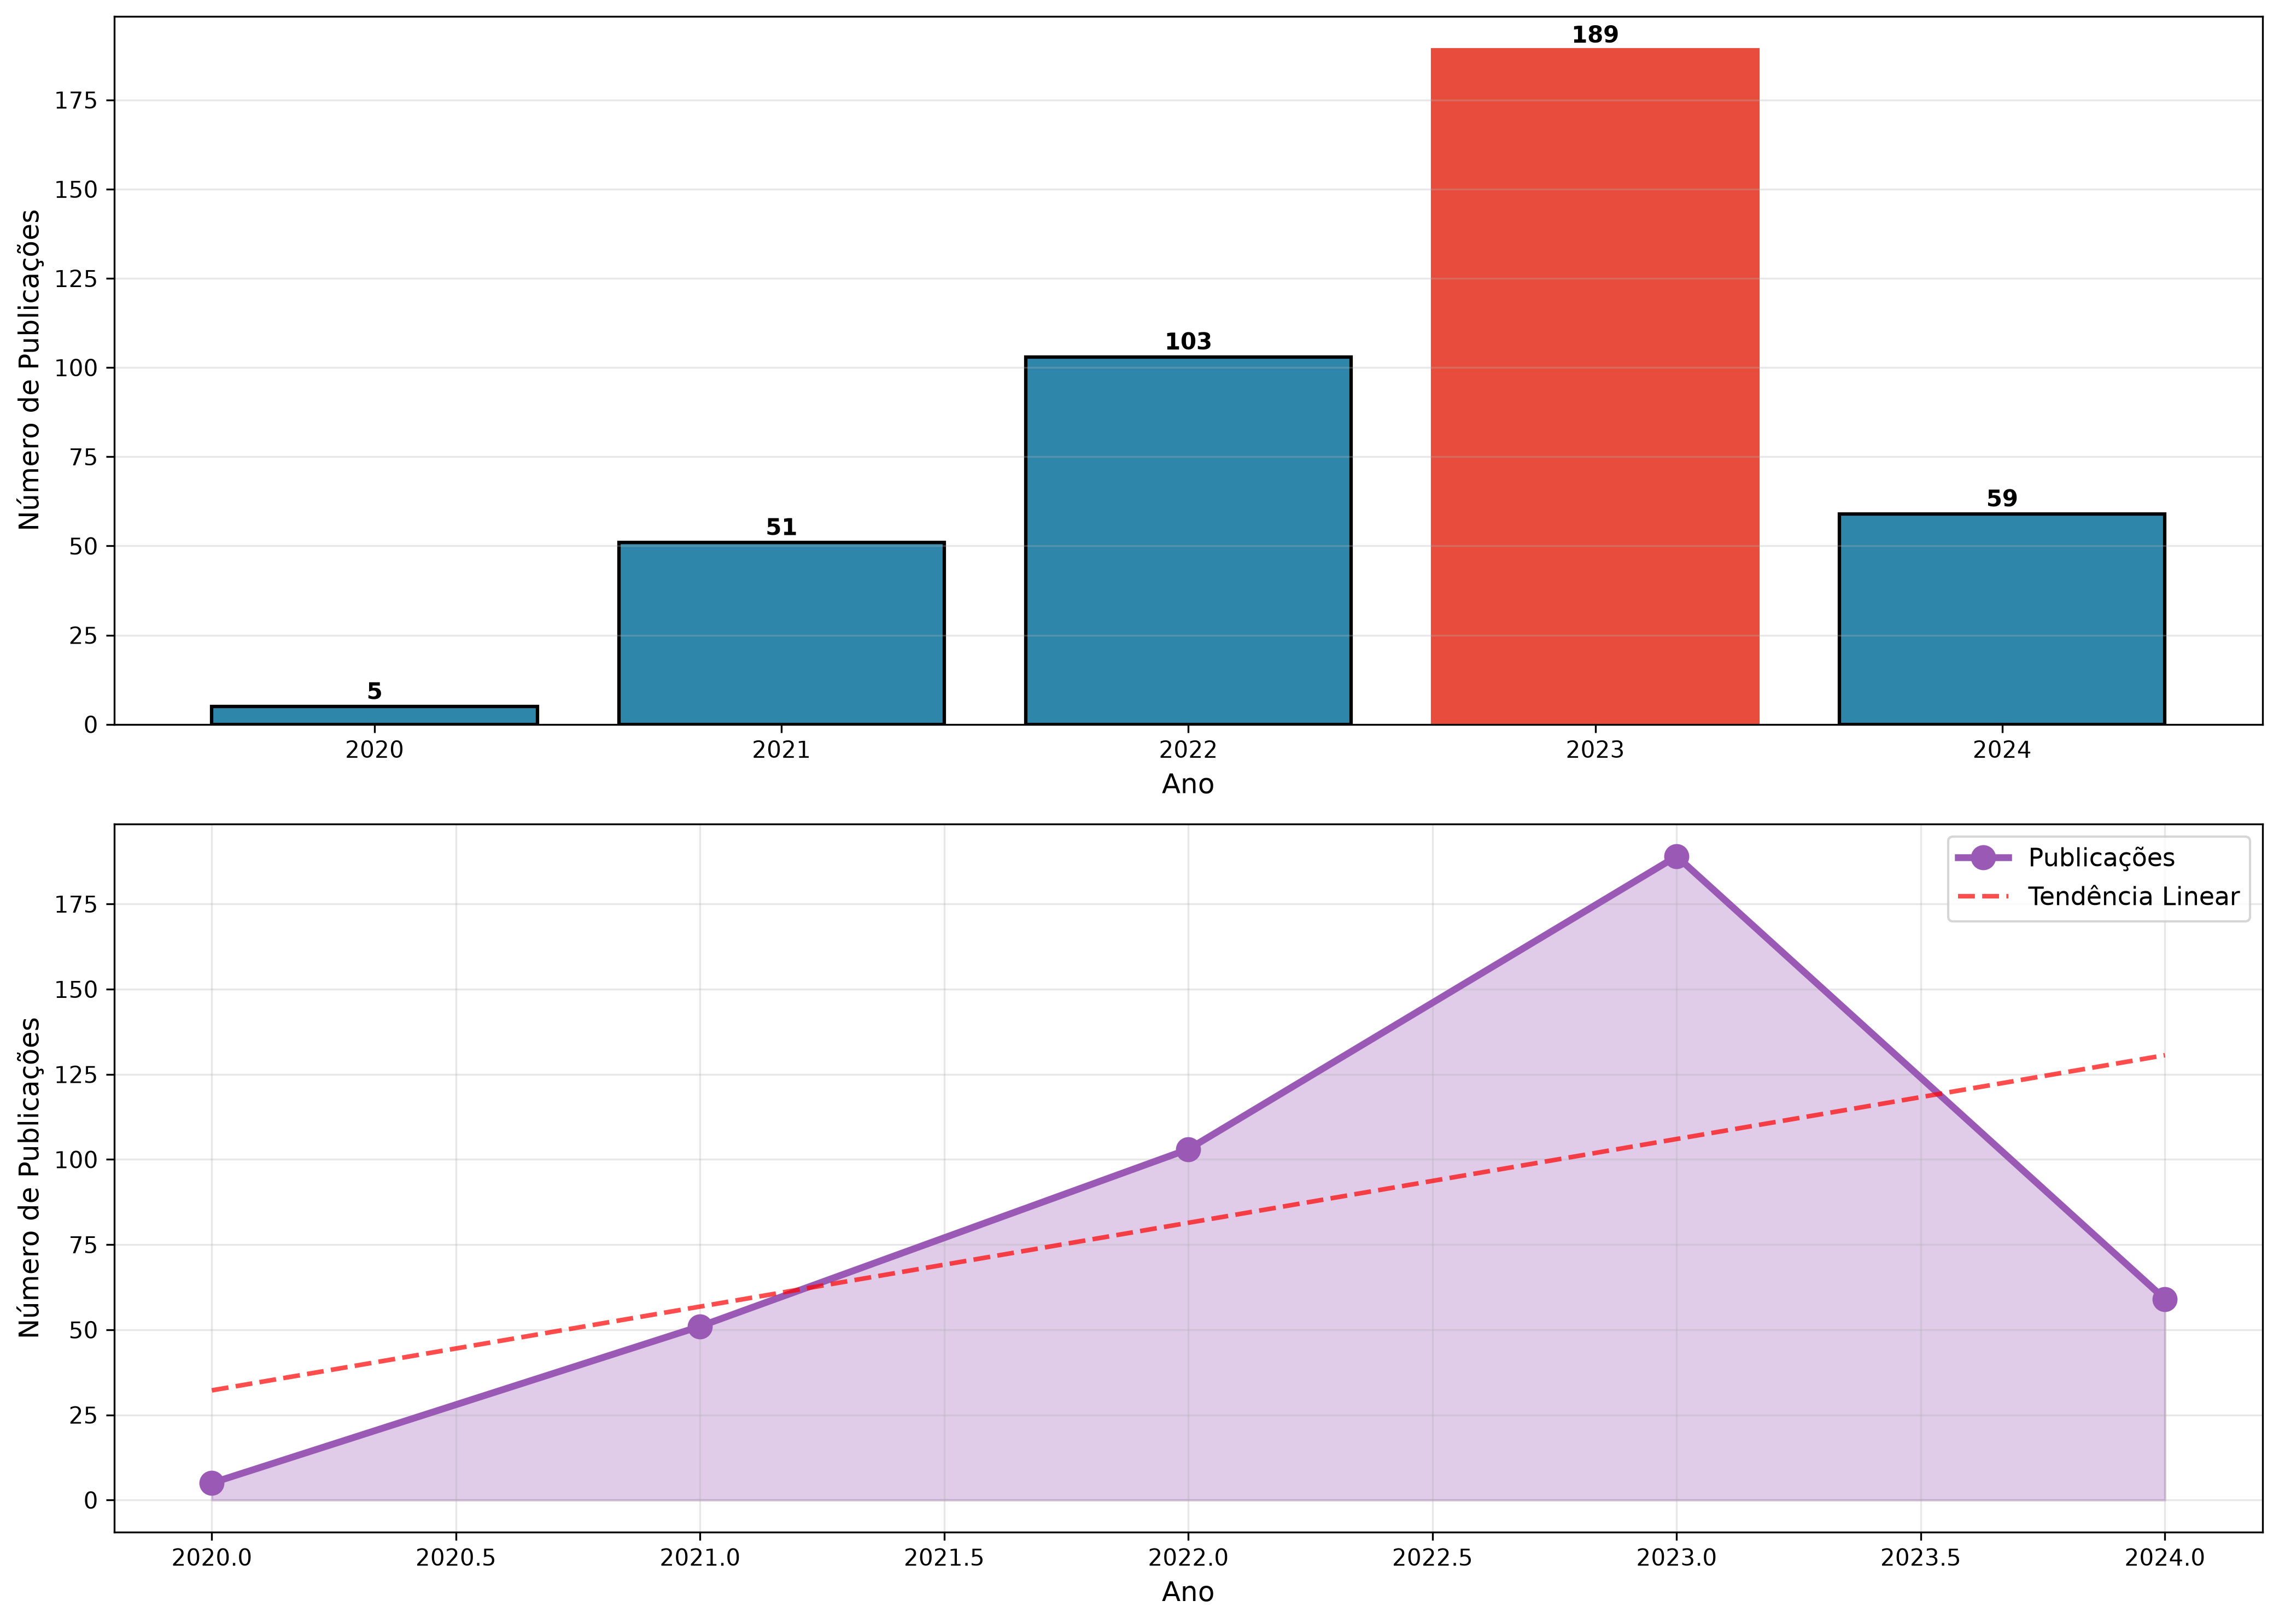
\includegraphics[width=0.95\textwidth]{3_evolucao_temporal_geral.png}
\caption[Evolução anual e tendência de crescimento]{%
\textbf{Evolução anual de publicações e tendência de crescimento do C4AI.}
\emph{Painel superior:} número absoluto de publicações por ano, com o ano de pico
(\textbf{2023}, \num{313} publicações) destacado em vermelho. Observa-se o
crescimento acelerado de 2020 (\num{7}) a 2023, seguido de queda acentuada em
2024 (\num{66}). \emph{Painel inferior:} a mesma série com a curva de
\emph{tendência linear} (linha tracejada vermelha) sobreposta; a tendência
permanece positiva, mas a queda de 2024 sugere um possível artefato de coleta
incompleta dos dados desse ano, e não necessariamente uma redução real da
produção.}
\label{fig:temporal}
\end{figure}

% ── Figura 4: Heatmap ─────────────────────────────────────────────────────────
\begin{figure}[H]
\centering
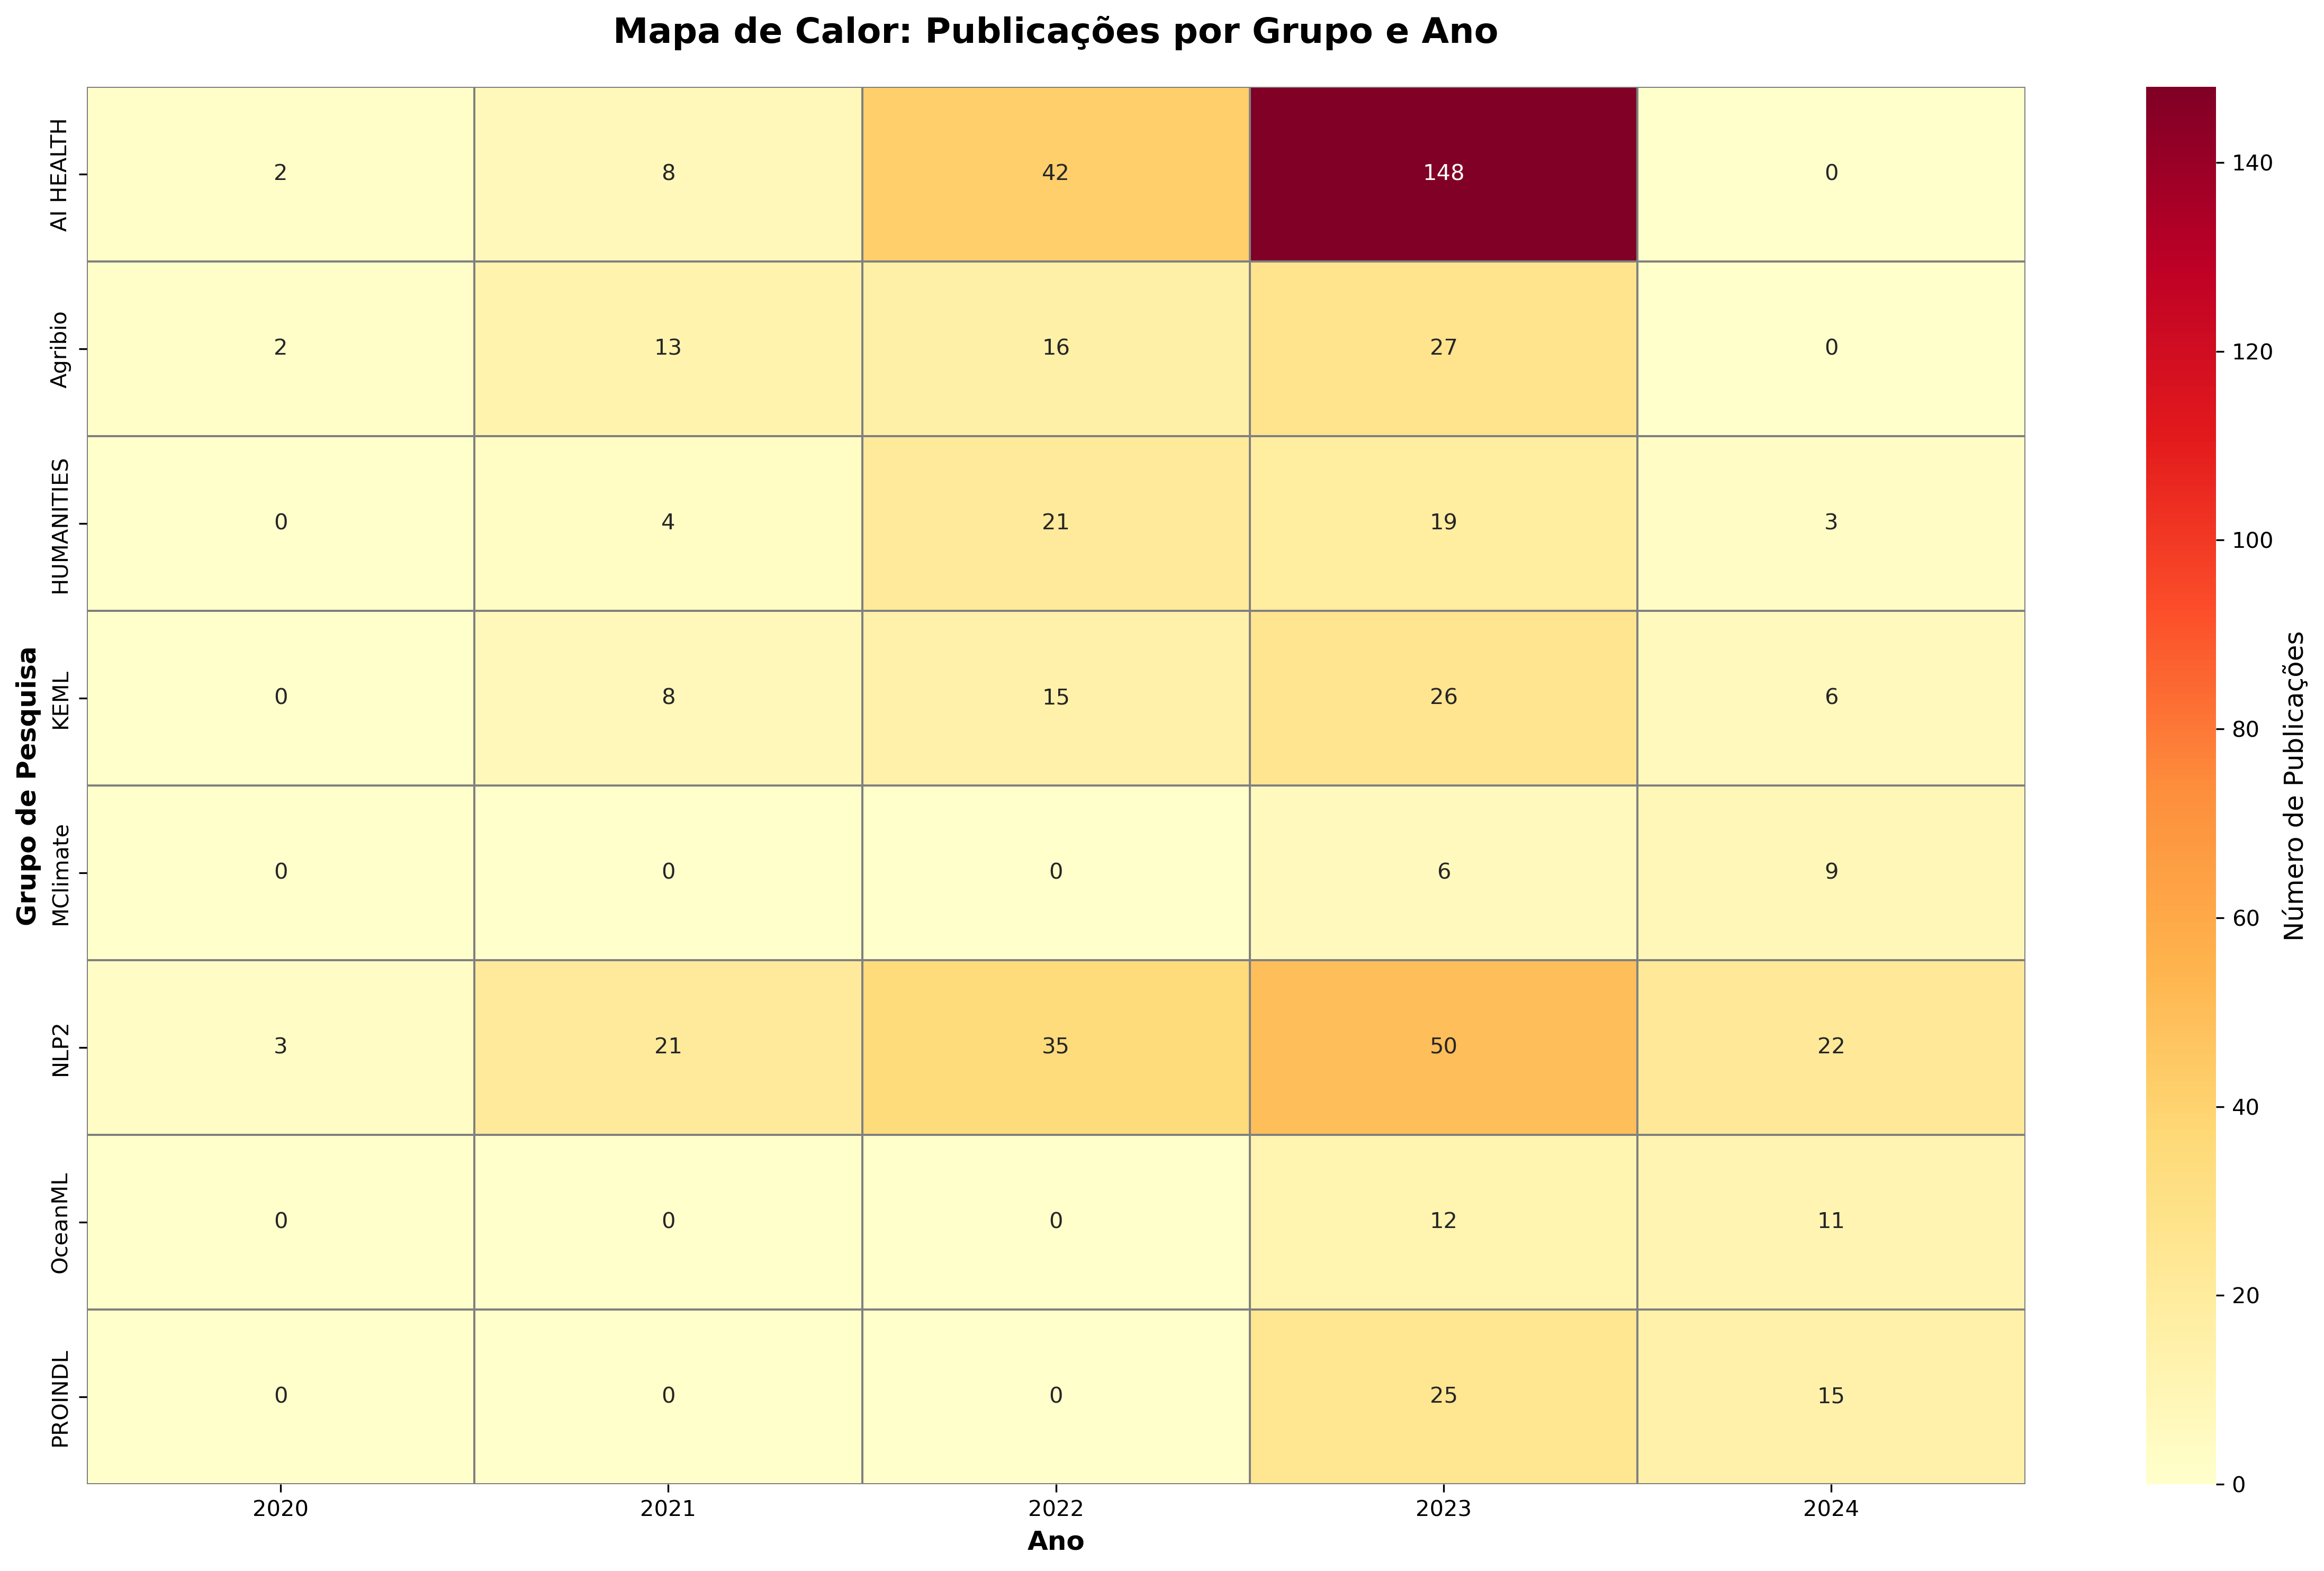
\includegraphics[width=0.95\textwidth]{4_heatmap_grupo_ano.png}
\caption[Mapa de calor grupo \texttimes{} ano]{%
\textbf{Mapa de calor: publicações por grupo e ano.}
Cada célula indica o número de publicações de um grupo em um determinado ano; a
intensidade da cor é proporcional ao volume. A célula mais intensa corresponde a
\textbf{AI HEALTH em 2023} (\num{148} publicações), responsável por boa parte do
pico geral observado na Figura~\ref{fig:temporal}. O mapa também revela a entrada
mais tardia de alguns grupos --- MClimate, OceanML e PROINDL só registram
publicações a partir de 2023 ---, enquanto AI HEALTH e NLP2 mantêm produção em
todo o período.}
\label{fig:heatmap}
\end{figure}

% ── Figura 5: Linhas todos os grupos ──────────────────────────────────────────
\begin{figure}[H]
\centering
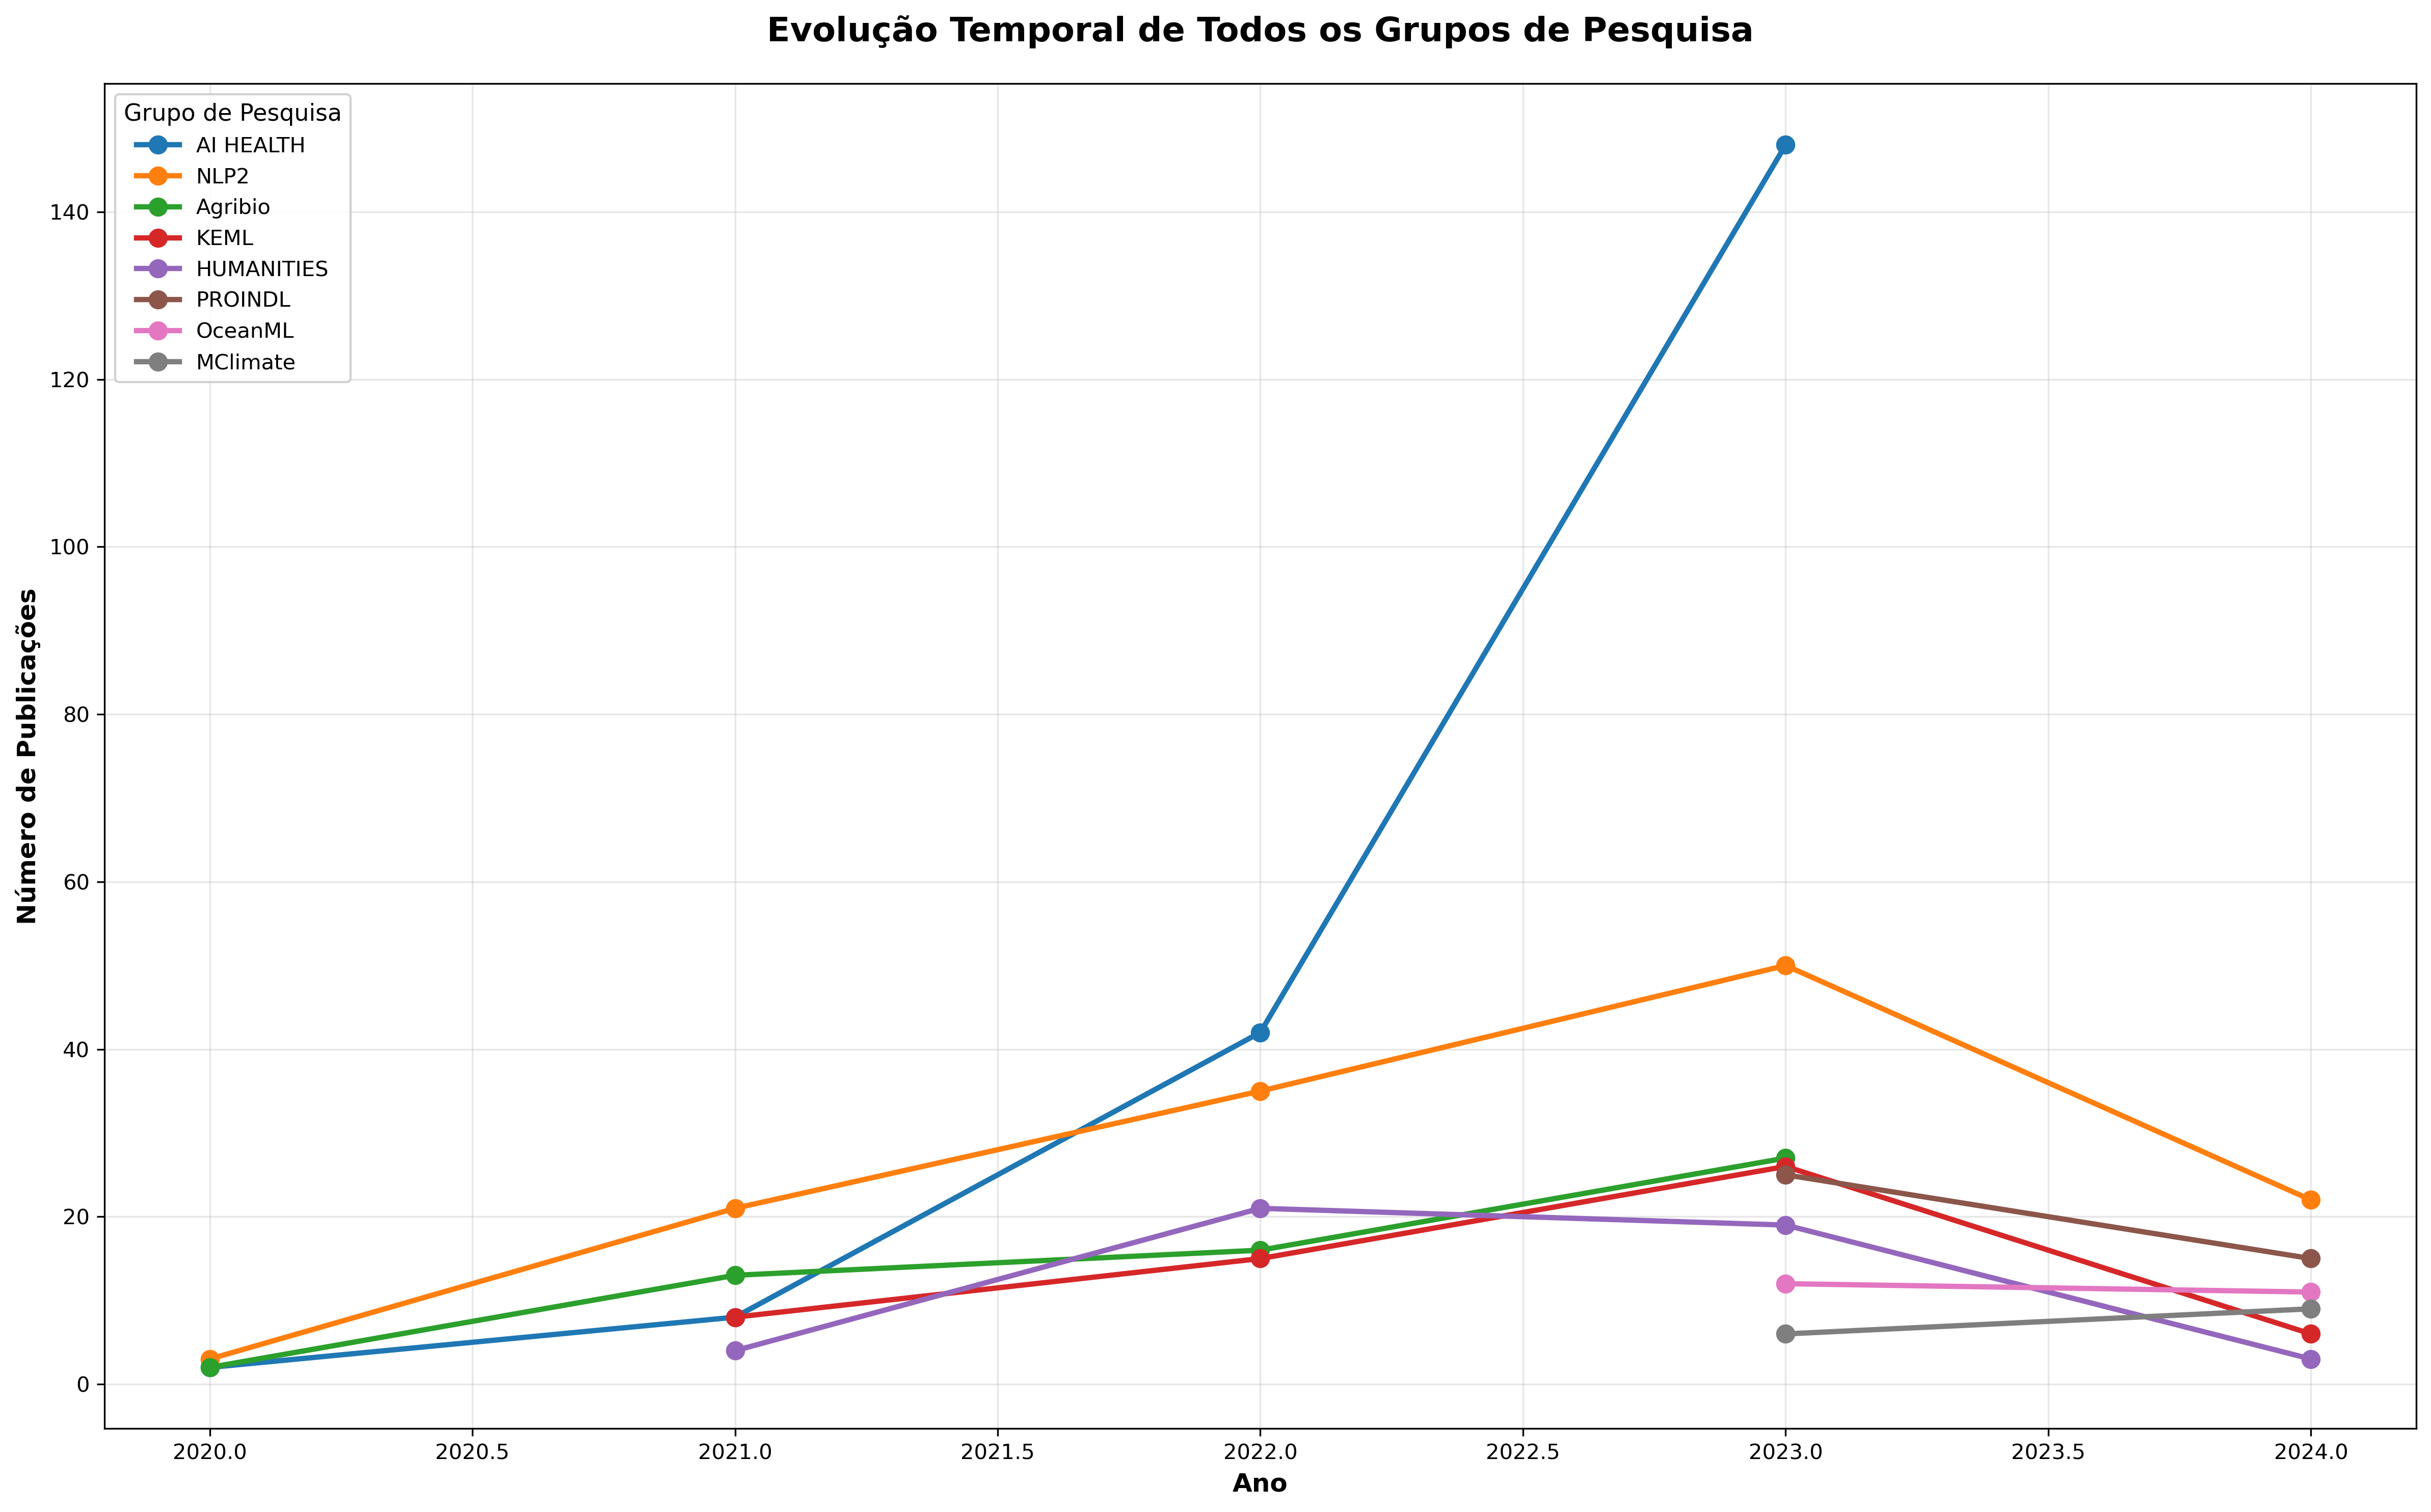
\includegraphics[width=0.95\textwidth]{5_evolucao_todos_grupos.png}
\caption[Evolução temporal de todos os grupos]{%
\textbf{Evolução temporal de todos os grupos de pesquisa.}
Séries anuais sobrepostas para os oito grupos. Destaca-se a trajetória de
\textbf{AI HEALTH} (linha azul), com crescimento exponencial até 2023, em
contraste com as trajetórias mais estáveis dos demais grupos. A convergência das
linhas em 2024 reflete tanto a maturação dos grupos menores quanto a já mencionada
provável incompletude dos dados do último ano.}
\label{fig:linhas}
\end{figure}

% ── Figura 7: Comparação top grupos ───────────────────────────────────────────
\begin{figure}[H]
\centering
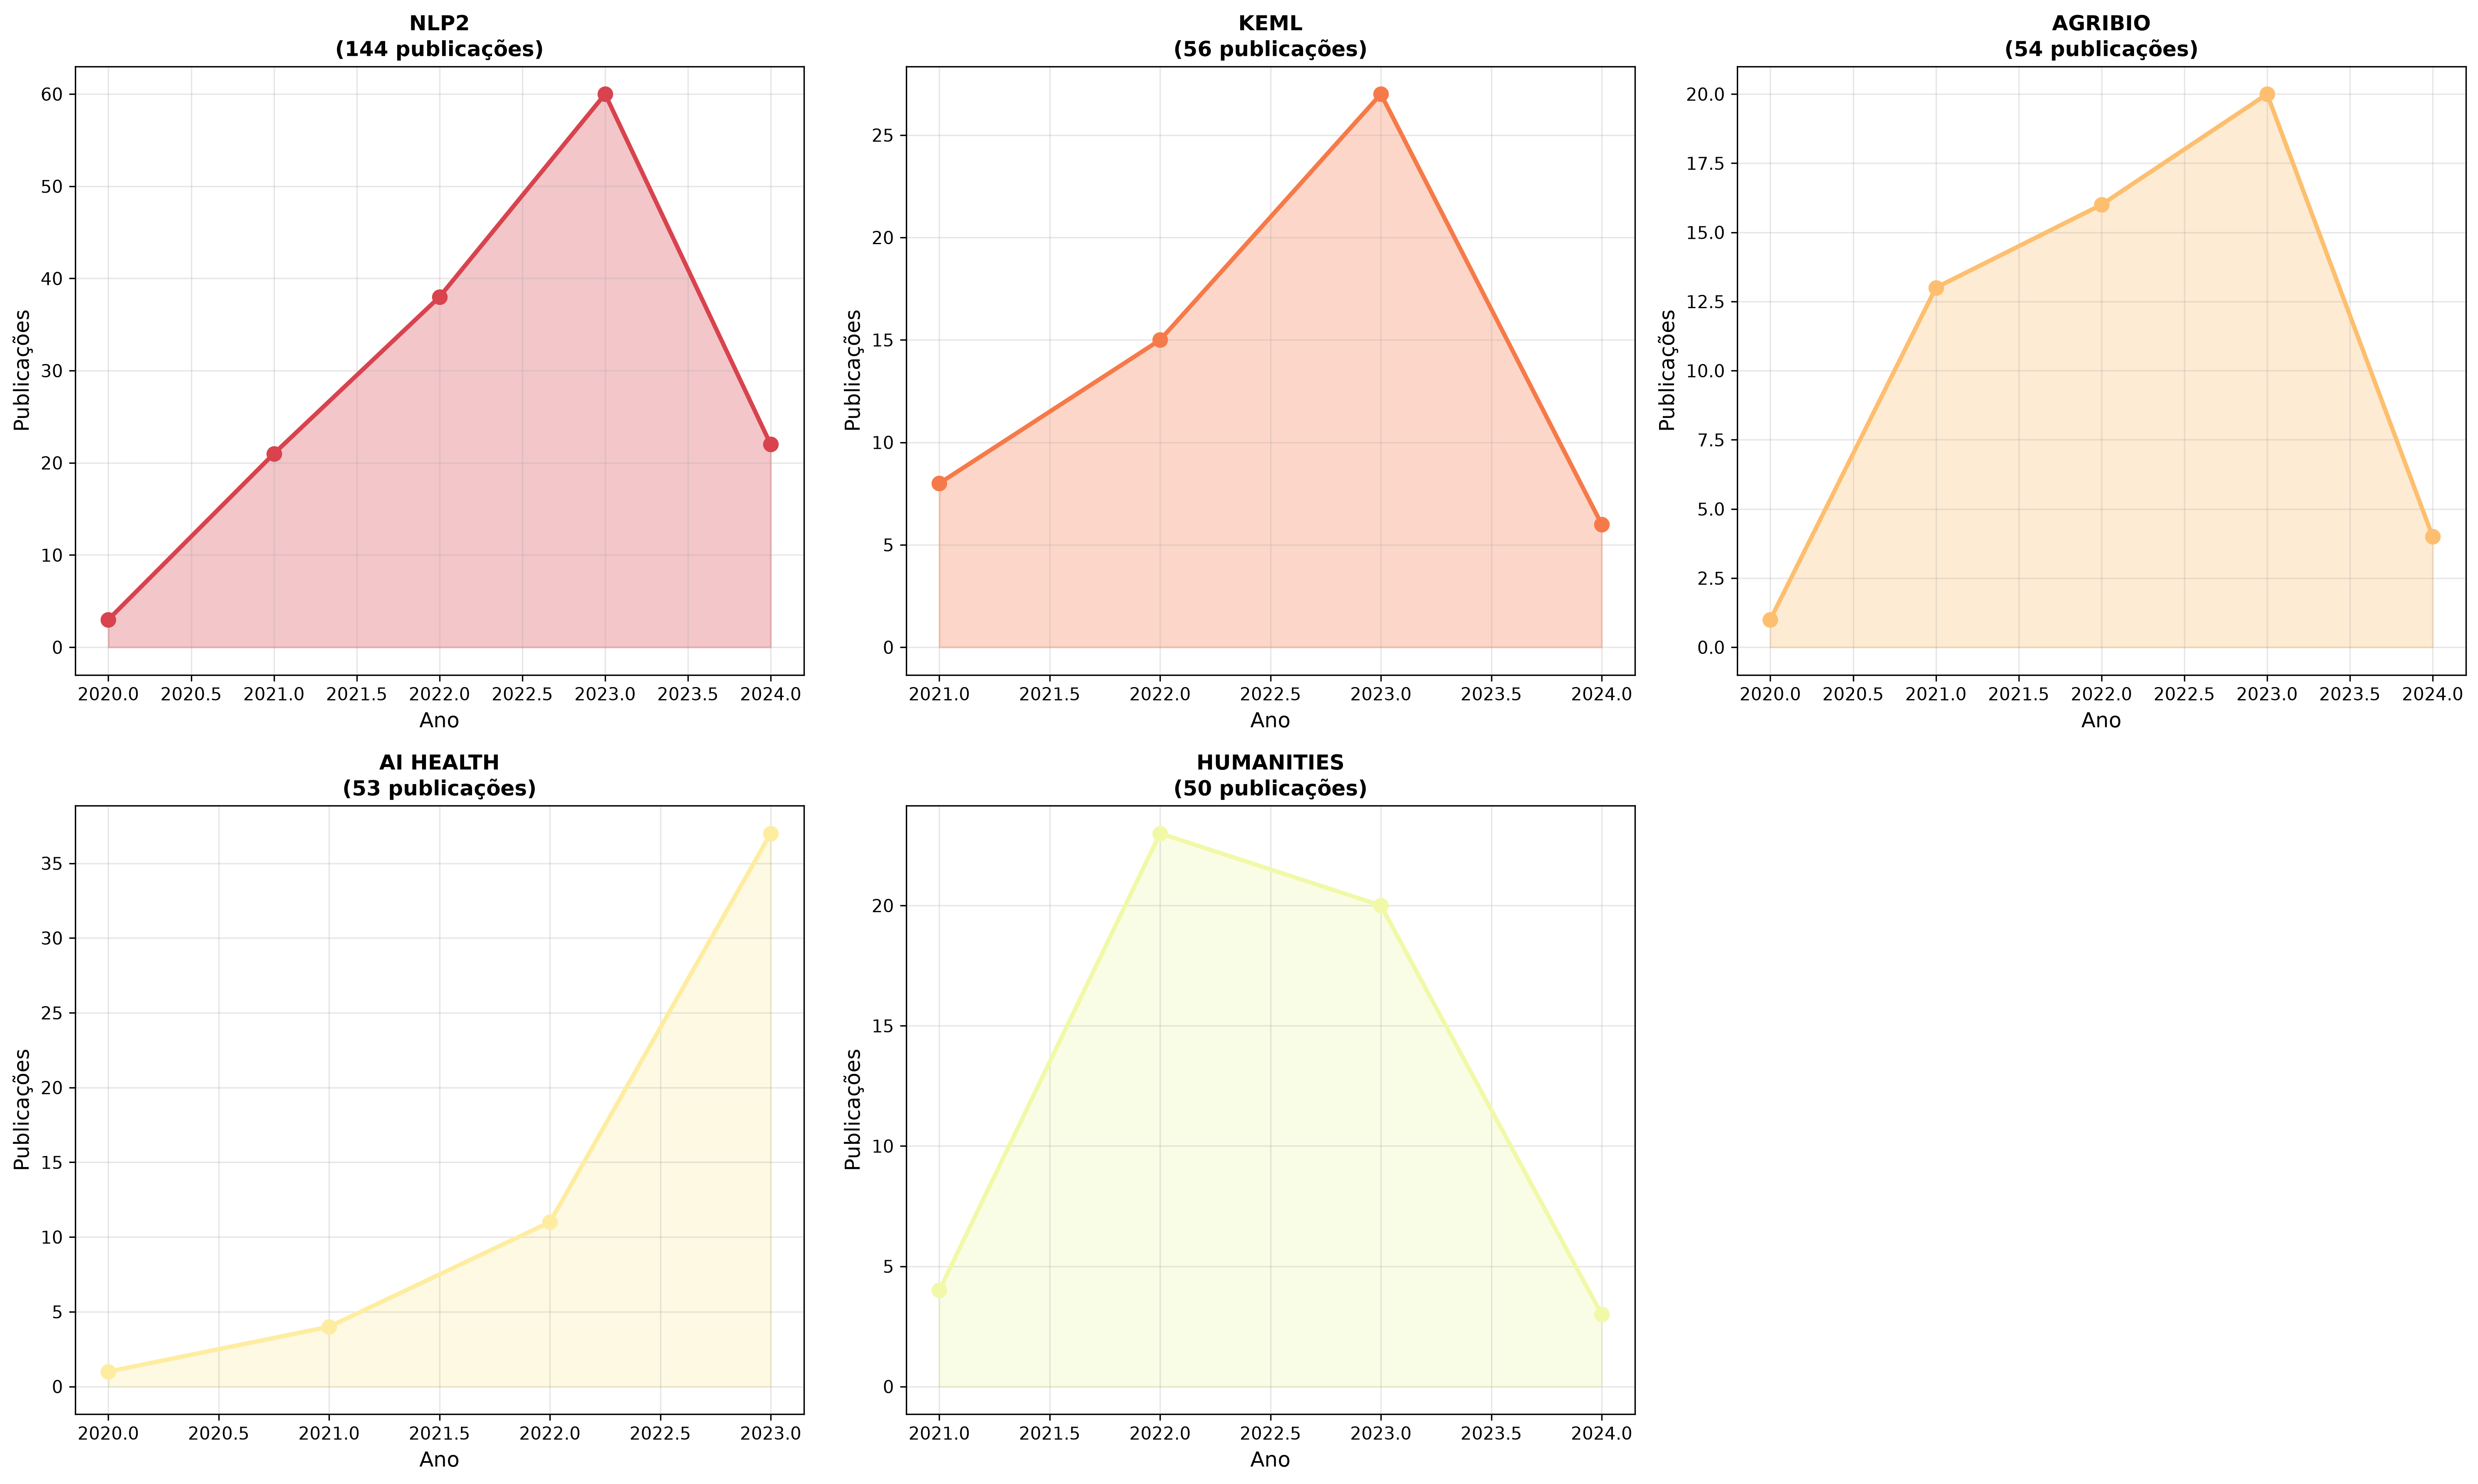
\includegraphics[width=0.95\textwidth]{7_comparacao_top_grupos.png}
\caption[Evolução temporal dos principais grupos]{%
\textbf{Evolução temporal dos cinco principais grupos.}
Painéis individuais (\emph{small multiples}) com a série anual de cada um dos
cinco grupos mais produtivos, permitindo comparar perfis de crescimento sem a
sobreposição da Figura~\ref{fig:linhas}. AI HEALTH (\num{200} pubs) e NLP2
(\num{131} pubs) apresentam crescimento sustentado até 2023; KEML e HUMANITIES
exibem perfis em forma de pico, com máximo em 2023 e 2022, respectivamente; e
Agribio mantém crescimento gradual e consistente.}
\label{fig:topgrupos}
\end{figure}

% ── Figura 8: Composição empilhada ────────────────────────────────────────────
\begin{figure}[H]
\centering
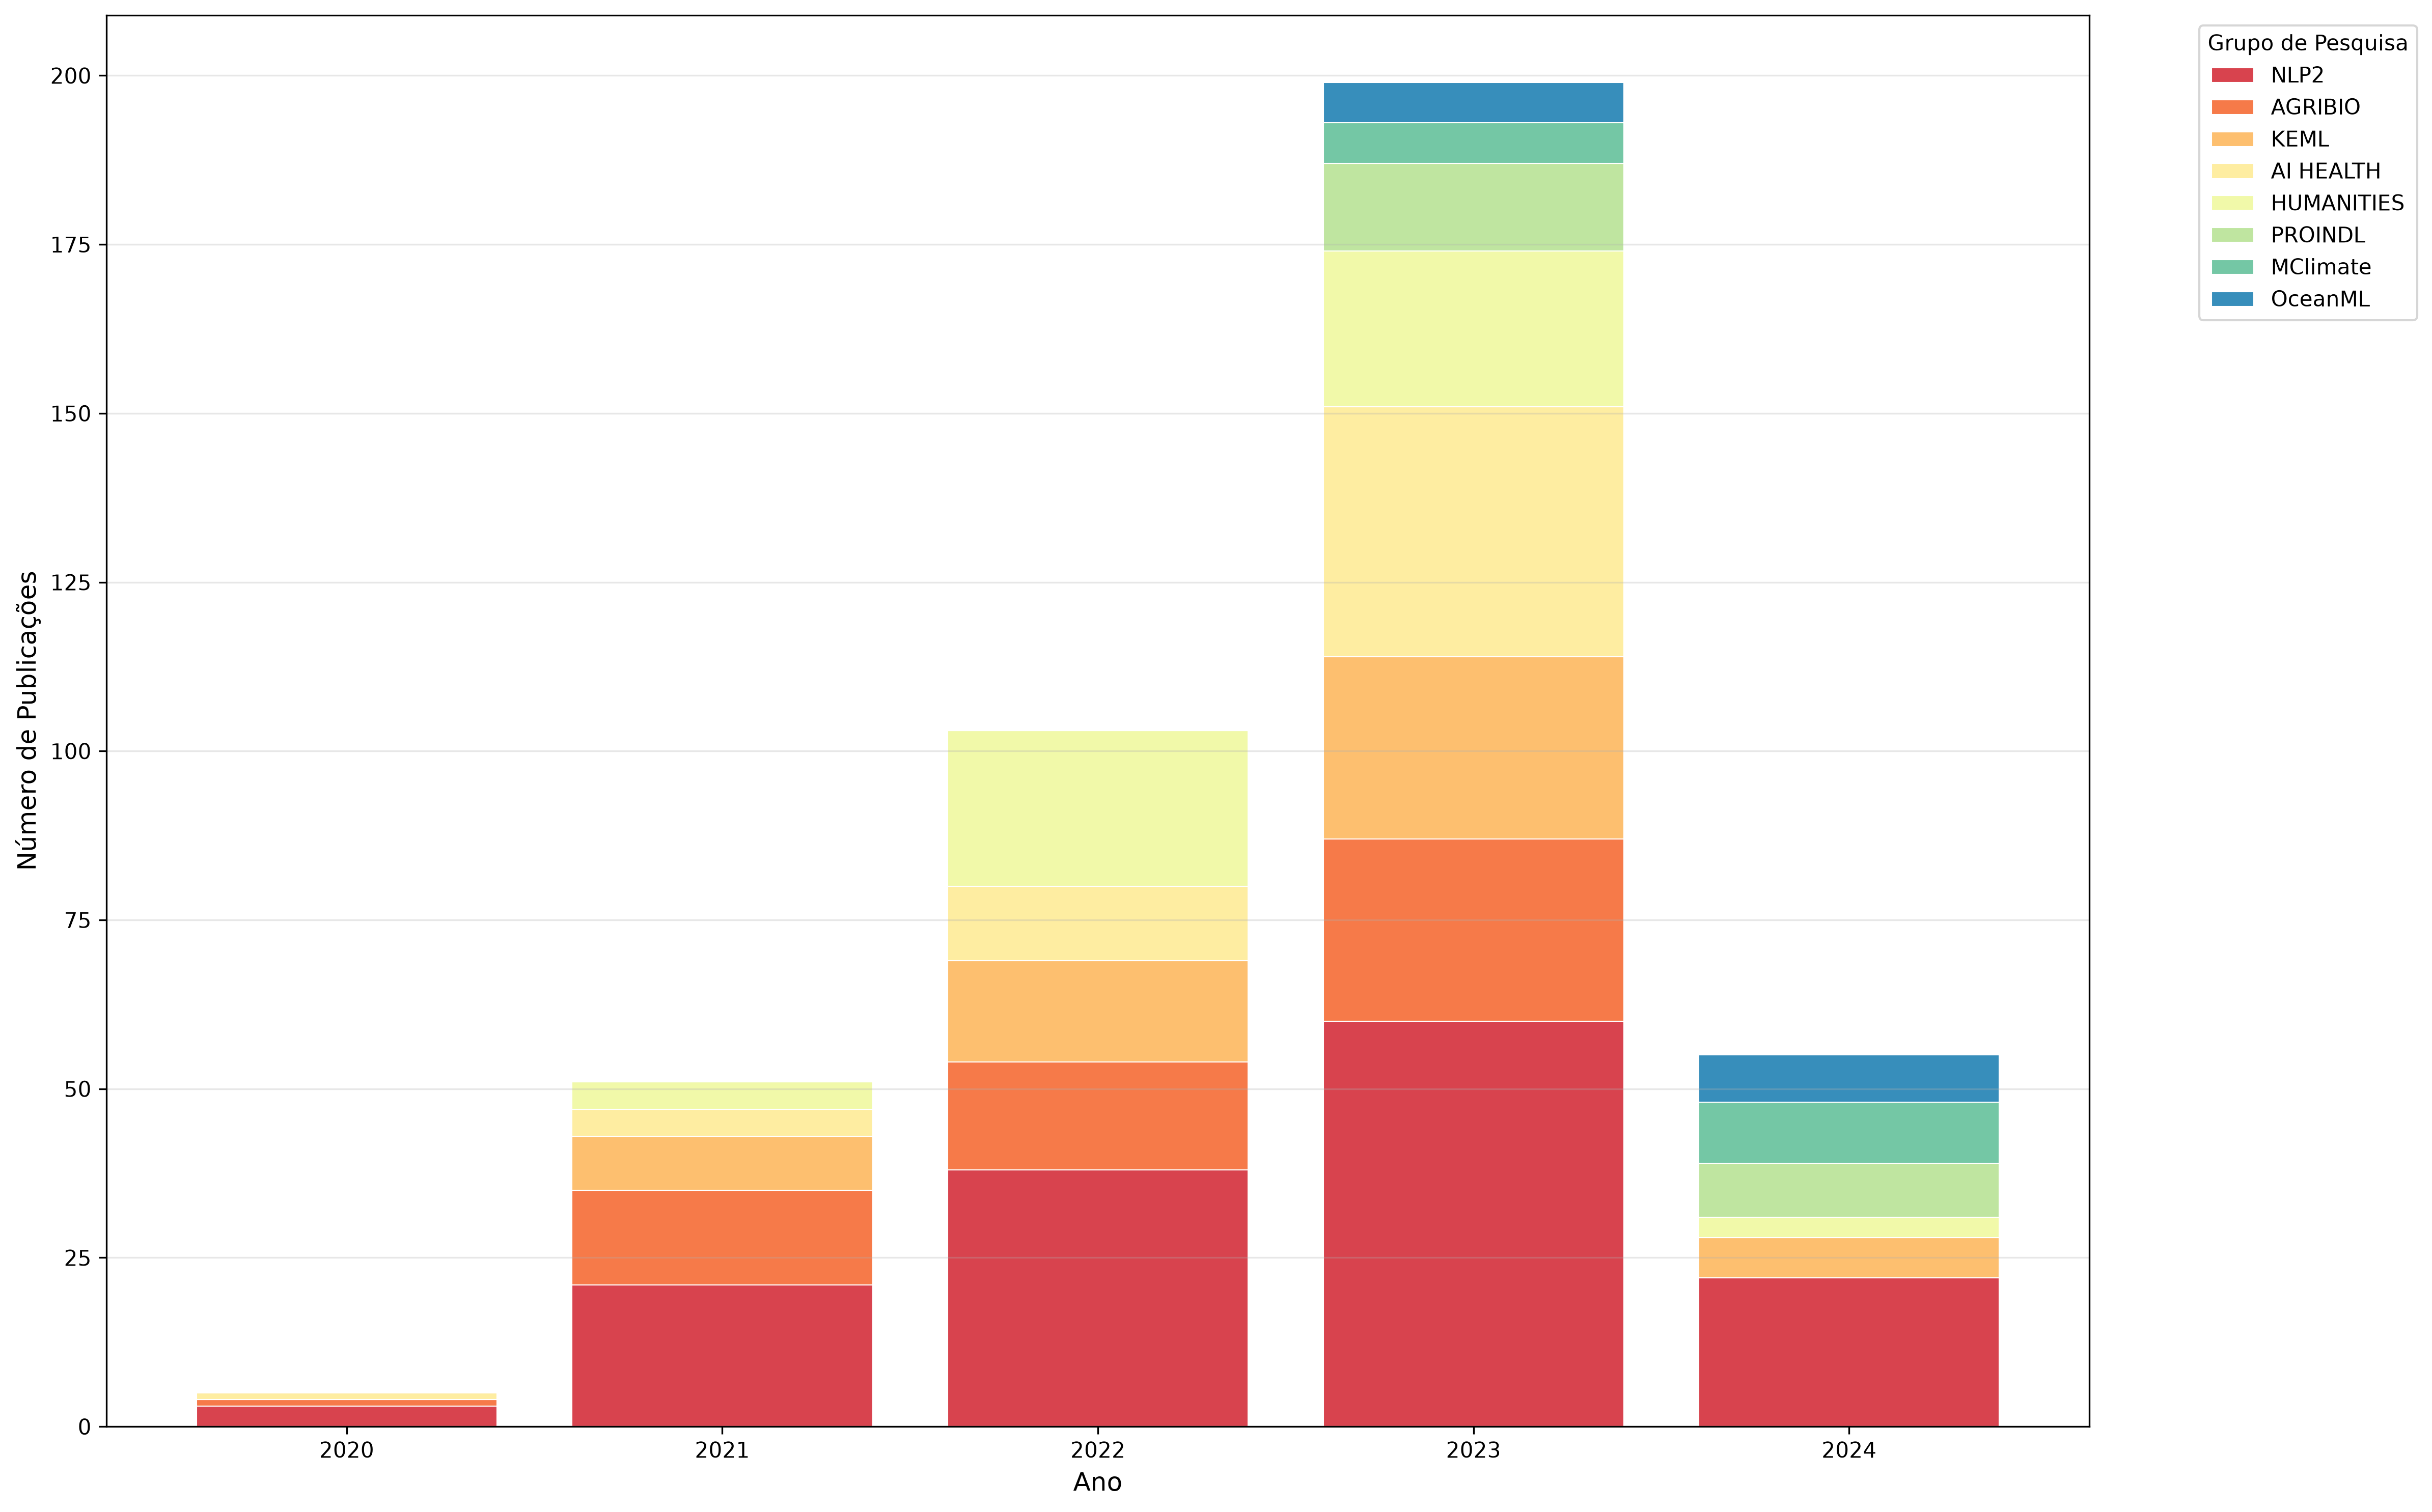
\includegraphics[width=0.95\textwidth]{8_composicao_temporal.png}
\caption[Composição temporal empilhada]{%
\textbf{Composição de publicações por grupo ao longo do tempo.}
Barras empilhadas que decompõem o total anual segundo a contribuição de cada
grupo. Além de confirmar o pico de 2023, o gráfico evidencia a mudança na
composição da produção: nos primeiros anos a produção é dominada por NLP2 e
Agribio, ao passo que, a partir de 2022--2023, \textbf{AI HEALTH} (faixa
vermelha) passa a responder pela maior parcela do volume anual.}
\label{fig:empilhado}
\end{figure}

% ==============================================================================
\section{Produtividade e concentração}
% ==============================================================================

% ── Figura 6: Produtividade ───────────────────────────────────────────────────
\begin{figure}[H]
\centering
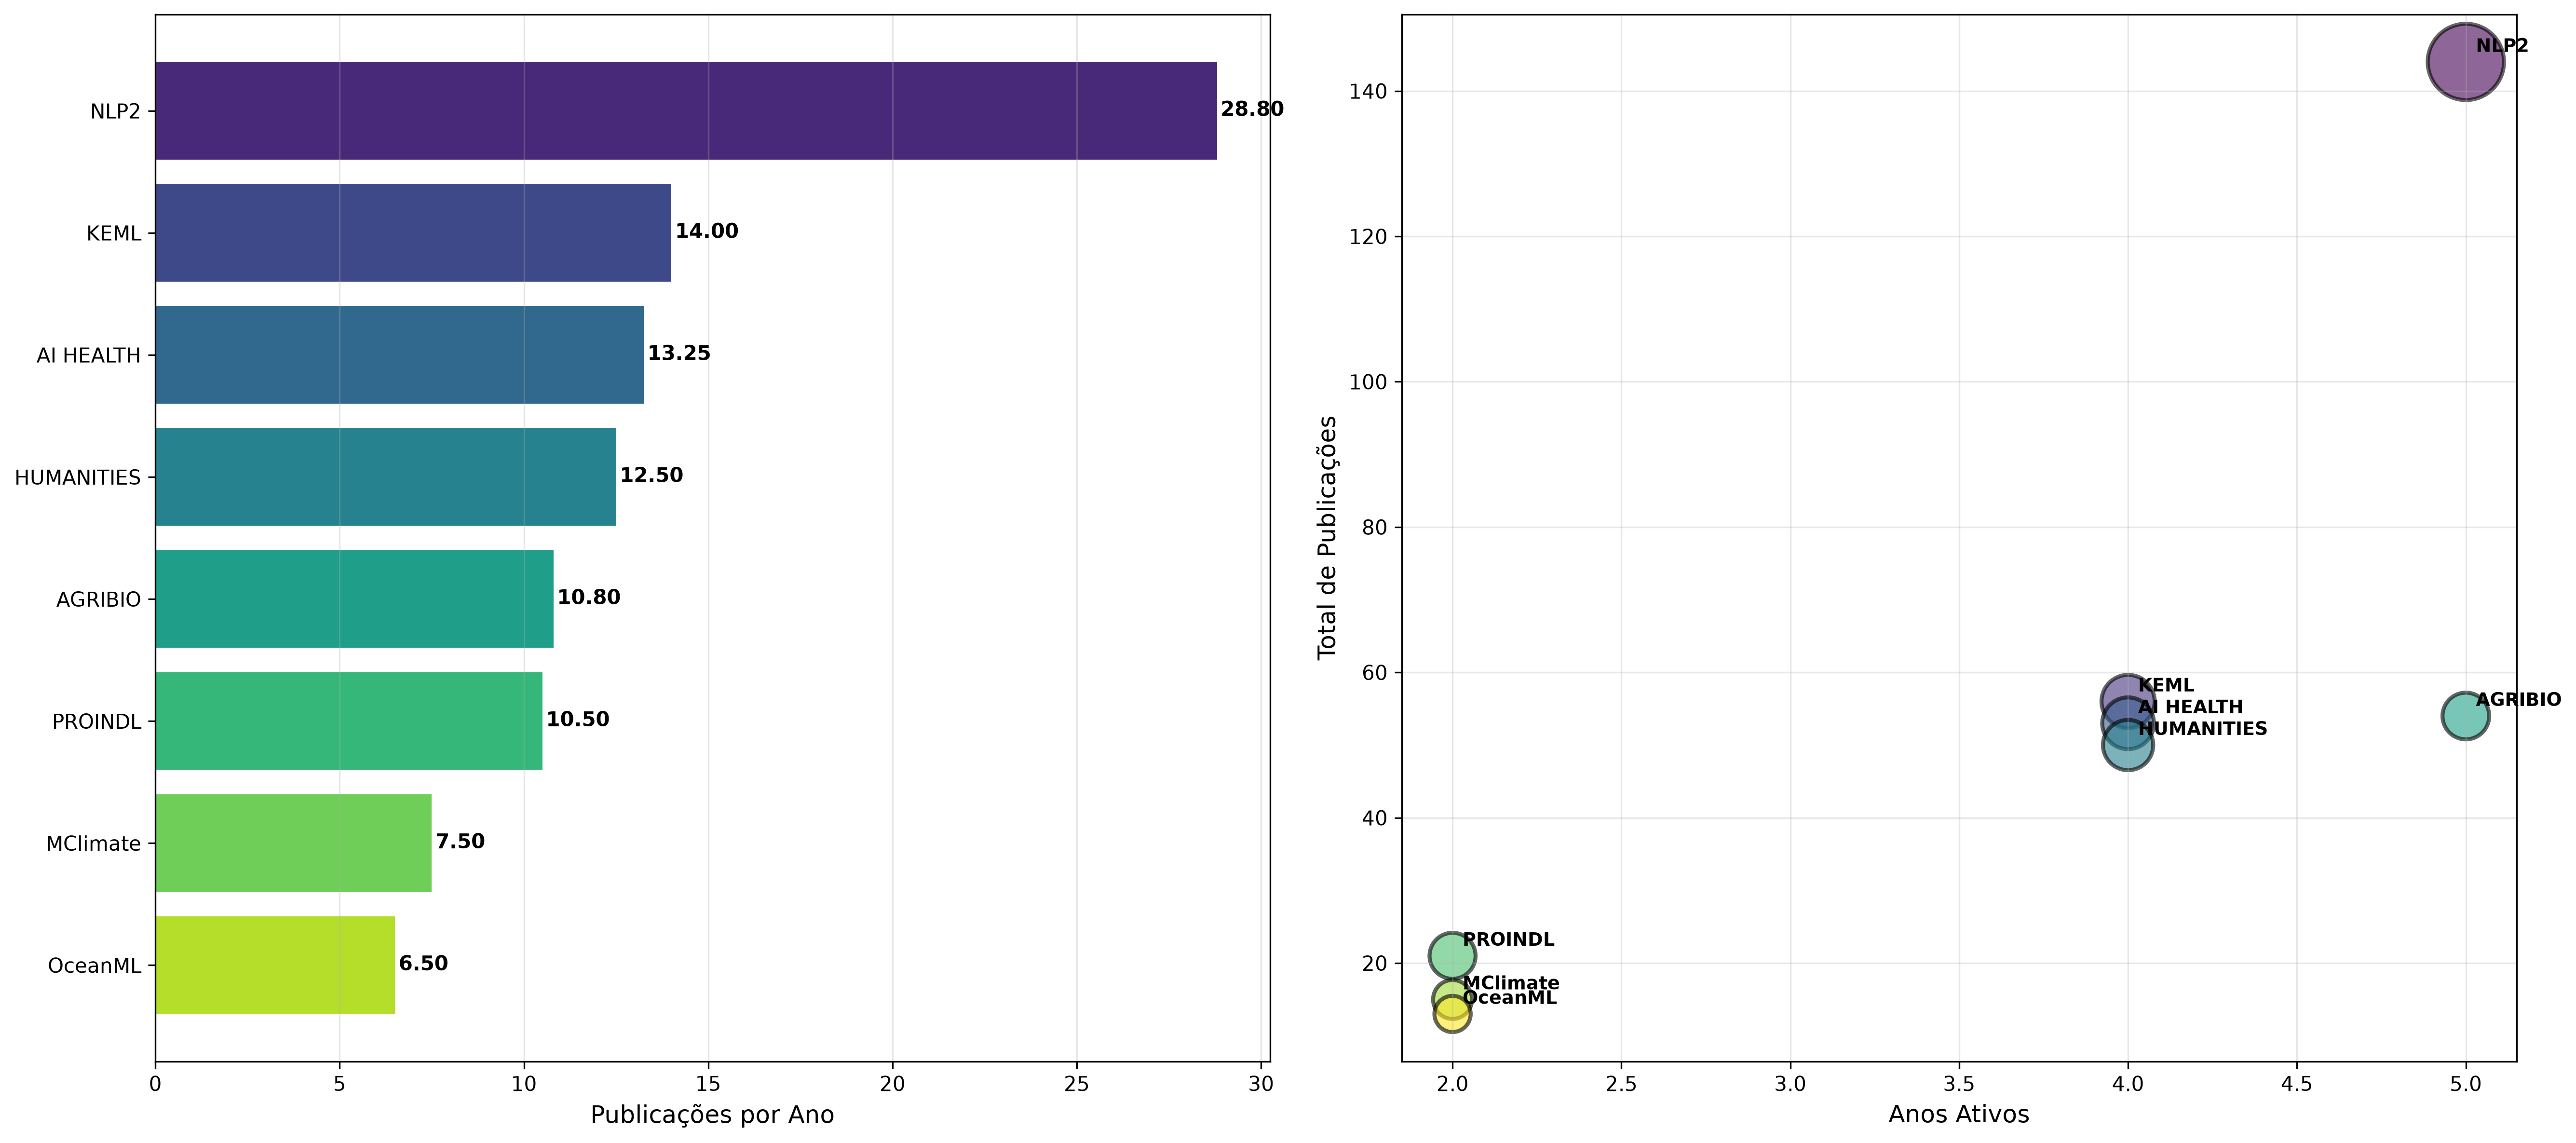
\includegraphics[width=0.95\textwidth]{6_produtividade_grupos.png}
\caption[Taxa de produtividade por grupo]{%
\textbf{Taxa de produtividade e relação produção \texttimes{} tempo de atividade.}
\emph{Painel esquerdo:} taxa de produtividade (publicações por ano de atividade)
por grupo; AI HEALTH lidera com \num{50.00} pubs/ano, seguido por NLP2
(\num{26.20}) e PROINDL (\num{20.00}). \emph{Painel direito:} dispersão entre o
número de anos ativos (eixo \textit{x}) e o total de publicações (eixo \textit{y}),
em que o tamanho de cada círculo é proporcional à taxa de produtividade.
Grupos como PROINDL alcançam alta produtividade apesar do curto período de
atividade, enquanto NLP2 combina longevidade e volume elevado.}
\label{fig:produtividade}
\end{figure}

\subsection{Índice de concentração (HHI)}

O grau de concentração da produção foi quantificado pelo índice
Herfindahl--Hirschman (HHI), definido como a soma dos quadrados das participações
percentuais de cada grupo:
%
\begin{equation}
\mathrm{HHI} = \sum_{i=1}^{n} s_i^{2} \times 10\,000,
\qquad s_i = \frac{\text{publicações do grupo } i}{\text{total de publicações}}.
\end{equation}
%
O valor obtido foi de \textbf{HHI~$\approx$~\num{2104}}, situado na faixa
\emph{moderada} (\num{1500} a \num{2500}). Esse resultado é coerente com a
observação de que os três maiores grupos concentram \SI{68.4}{\percent} da
produção total, configurando um cenário de produção desigual, porém ainda não
plenamente monopolizado por um único grupo.

% ==============================================================================
\section{Considerações finais}
% ==============================================================================

A produção acadêmica do C4AI no período 2020--2024 caracteriza-se por:
\begin{itemize}
    \item \textbf{Forte concentração:} AI HEALTH e NLP2 respondem por
          \SI{58.1}{\percent} das publicações; os três maiores grupos, por
          \SI{68.4}{\percent} (HHI moderado $\approx$ \num{2104}).
    \item \textbf{Crescimento acelerado até 2023:} o volume anual saltou de
          \num{7} publicações em 2020 para \num{313} em 2023, impulsionado
          sobretudo pelo grupo AI HEALTH.
    \item \textbf{Queda aparente em 2024:} provavelmente associada à coleta
          incompleta dos dados do último ano, o que recomenda cautela na
          interpretação dessa redução.
    \item \textbf{Heterogeneidade de trajetórias:} convivem grupos de
          crescimento sustentado (AI HEALTH, NLP2, Agribio) com grupos de
          entrada recente e produção concentrada em poucos anos (MClimate,
          OceanML, PROINDL).
\end{itemize}

\noindent
As figuras e os indicadores aqui apresentados foram gerados automaticamente pelo
\emph{script} de análise (\texttt{analise\_publicacoes}) a partir do arquivo de
dados consolidado dos grupos de pesquisa do C4AI.

\end{document}
